\documentclass[german]{uebung}

\usepackage{uebung-meta}
\usepackage{enumitem}
\usepackage{amssymb}
\usepackage{multicol}
%%%%%%%%%%%%%%%%%%%%%%%%%%%%%%%%%%%%%%%%%%%%%%%%%%%%%%%%%%%%%%%%%%%%%%%%%%%%
% README
%%%%%%%%%%%%%%%%%%%%%%%%%%%%%%%%%%%%%%%%%%%%%%%%%%%%%%%%%%%%%%%%%%%%%%%%%%%%

% How to use this:
% 1. Add your data to uebung-meta.sty (you only need to do this once)
% 2. Copy this file and name it something useful
% 3. Set the assignment to the right value
% 4. Use the exercise enviroment to separate your solutions for the different exercises from each other.

% DO NOT CHANGE uebung.cls! If you need more packages just add a new \usepackage somewhere in this file before the \begin{document}

% The commands
% \div and \grad are provided by uebung.cls

% The environment "exercise" takes one parameter (the exercise number). 
% This way you can skip exercises if you like. Example:
% 
% \assignment{3}
% \begin{exercise}{8}
% ...
% \end{exercise}
% 
% The solution to exercise 3.8 (3rd assignment, 8th exercise) goes where 
% the dots are.

% If the total page number shows up as ?? in the footer you need to compile a second time.

% Which assignment is this?
\assignment{1}


\begin{document}

\begin{exercise}{1}
	\begin{enumerate}[label=(\alph*)]
		\item Definitionsbereich $x \in \mathbb{R}$\\Differenzierbar, da $f'(x)$ an allen Stellen definiert
			\begin{flalign*}
				f(x) &= x^3 - x + 8&\\
				f'(x) &= 3x^2 - 1&
		      \end{flalign*}

	      \item Definitionsbereich $x \in \mathbb{R}\backslash\{0\}$\\ Nicht differenzierbar, da $f'(x)$ an Stelle $x=0$ nicht definiert
			\begin{flalign*}
				f(x) &= \frac{1}{2x}&\\
				f'(x) &= \frac{2}{4x^2}&
		      \end{flalign*}
	      
	      \item Definitionsbereich $x \in \mathbb{R}$\\ Differenzierbar, da $f'(x)$ an allen Stellen definiert
			\begin{flalign*}
				f(x) &= 3 \cdot \sin(2x)&\\
				f'(x) &= 6 \cdot \cos(2x)&
		      \end{flalign*}
	      
	      \item Definitionsbereich $x \in \mathbb{R}$\\ Nicht differenzierbar, da $f'(x)$ an Stelle $x=0$ nicht definiert
			\begin{flalign*}
				f(x) &= |2x|&\\
				     &= 2 \cdot \sqrt{(x^2)}&\\
				f'(x) &= 2 \cdot \frac{x}{\sqrt{x^2}}&
		      \end{flalign*}

	\end{enumerate}
\end{exercise}

\begin{exercise}{2}
	\begin{enumerate}[label=(\alph*)]
		\item \begin{flalign*}
				grad f(x) &= \nabla f(x_1, x_2) &\\
					  &= \begin{pmatrix}
						\frac{\delta f}{\delta x_1}(x_1, x_2) \\ \\
						\frac{\delta f}{\delta x_2}(x_1, x_2)
					     \end{pmatrix}&\\
					  &=  \begin{pmatrix}
						  6x_{1}^{2} + 10x_{1}x_{2} - 2x_{2}^{2}\\ \\
						  5x_{1}^{2} - 4x_{1}x_{2} + 2x_{2}	
					     \end{pmatrix}&\\
		      \end{flalign*}

		\item \begin{flalign*}
				f(x)	  &= e^{2||x||^{2}}&\\
					  &= e^{g(x)}&\\
				f'(x)	  &= g'(x) \cdot e^{g(x)}&\\
				g(x)      &= 2||x||^{2}&\\
					  &= 2{\sqrt{x_1^{2} + ... + x_n^{2}}}^{2}\\
					  &= 2\cdot (x_1^{2} + ... + x_n^{2})&\\
					  &= 2x_1^{2} + ... + 2x_n^{2}&\\
  	\frac{\delta g}{\delta x_i}(x)	  &= 4x_i\\\\
				grad\; f(x) &= \nabla f(x_1,..., x_n) &\\
					  &= \begin{pmatrix}
						\frac{\delta f}{\delta x_1}(x_1,..., x_n) \\
						  ...\\
						\frac{\delta f}{\delta x_n}(x_1,..., x_n)
					     \end{pmatrix}&\\
					  &=  \begin{pmatrix}
						  4x_1\cdot e^{2||x||^{2}}\\ ... \\
						  4x_n\cdot e^{2||x||^{2}}\\
					     \end{pmatrix}&\\
		      \end{flalign*}
	\end{enumerate}
\end{exercise}

\begin{exercise}{3}
	\begin{enumerate}[label=(\alph*)]
		\item 
			\begin{flalign*}
				f(x)	    &= \begin{pmatrix}
					v_1(x_1, x_2)\\ v_2(x_1, x_2)
						\end{pmatrix}&\\
				\nabla f(x) &= \frac{\delta v_1}{\delta x_1}(x_1, x_2)
						+ \frac{\delta v_2}{\delta x_2}(x_1, x_2)&\\
					    &= 3 + 2x_2 + 5x_{2}^{4} + x_{1}^{2}
			\end{flalign*}

		\item 
			\begin{flalign*}
					f(x)&= \begin{pmatrix}
						v_1(x_1,...,x_n)\\ ... \\ v_n(x_1,...,x_n)
						\end{pmatrix}
						= \begin{pmatrix}
						2x_1\\ ... \\ 2x_n
						\end{pmatrix}&\\
				\nabla f(x) &= \sum_{i=1}^{n} \frac{\delta v_i}{\delta x_i} (x_1,...,x_i)&\\
					    &= \sum_{i=1}^{n} 2 = n \cdot 2
			\end{flalign*}

	\end{enumerate}
\end{exercise}


\begin{exercise}{4}
	\begin{enumerate}[label=(\alph*)]
		\item 

			$ \begin{pmatrix} 3 & 4 \\ 2 & 1 \end{pmatrix} $ \\
			\begin{flalign*}
				det \begin{pmatrix} (3-\lambda) & 4 \\ 2 & (1-\lambda) \end{pmatrix}
					&= (3-\lambda)(1-\lambda) - 4\cdot 2&\\
					&= \lambda^{2} -4\lambda - 5&
			\end{flalign*}
			Eigenwerte: $\lambda_{1} = 5, \lambda_{2} = -1 $\\

			Eigenvektor:\\
			\begin{multicols}{2}
			Sei $\lambda = 5$\\
			\begin{flalign*}
				(I)\quad  (3-\lambda)x + 4y &= 0&\\
				(II)\quad  2x + (1-\lambda)y &= 0&\\\\
				(I)\quad  -2x + 4y &= 0&\\
				(II)\quad\;\;\;  2x - 4y &= 0&\\\\
				\rightarrow x=2y
			\end{flalign*}
			L\"osungsmenge $L$:
			\begin{flalign*}
				L &= \left\{ a \cdot \begin{pmatrix} 2 \\ 1 \end{pmatrix} \middle| a \in \mathbb{R}\right\} &
			\end{flalign*}
			\columnbreak
			
			Sei $\lambda = -1$
			\begin{flalign*}
				(I)\quad  (3-\lambda)x + 4y &= 0&\\
				(II)\quad  2x + (1-\lambda)y &= 0&\\\\
				(I)\quad  4x + 4y &= 0&\\
				(II)\quad  2x + 2 &= 0&\\\\
				\rightarrow x=-y
			\end{flalign*}
			L\"osungsmenge $L$:
			\begin{flalign*}
				L &= \left\{ a \cdot \begin{pmatrix} 1 \\ -1 \end{pmatrix} \middle| a \in \mathbb{R}\right\} &
			\end{flalign*}
			
			\end{multicols}


		\item 
			$ \begin{pmatrix} -1 & 3 \\ 2 & -2 \end{pmatrix} $ \\
			\begin{flalign*}
				det \begin{pmatrix} (-1-\lambda) & 3 \\ 2 & (-2-\lambda) \end{pmatrix}
					&= (-1-\lambda)(-2-\lambda) - 2\cdot 3&\\
					&= \lambda^{2} +3\lambda - 4&
			\end{flalign*}
			Eigenwerte: $\lambda_{1} = 1, \lambda_{2} = -4 $\\
			\newpage
			Eigenvektor:\\
			\begin{multicols}{2}
			Sei $\lambda$ = 1\\
				\begin{flalign*}
					(I)\quad  (-1-\lambda)x + 3y &= 0&\\
					(II)\quad 2x + (-2 -\lambda)y &= 0&\\\\
					(I)\quad  -2x + 3y &= 0&\\
					(II)\quad\;\;\;  2x - 3y &= 0&\\
					\rightarrow x = \frac{3}{2}y
				\end{flalign*}
			L\"osungsmenge $L$:
				\begin{flalign*}
					L & \left\{ a \cdot \begin{pmatrix} \frac{3}{2} \\ 1 \end{pmatrix} \middle| a \in \mathbb{R} \right\}&
				\end{flalign*}\columnbreak\\
			Sei $\lambda$ = -4
				\begin{flalign*}
					(I)\quad  (-1-\lambda)x + 3y = 0&\\
					(II)\quad 2x + (-2-\lambda)y = 0&\\\\
					(I)\quad  3x + 3y = 0&\\
					(II)\quad 2x + 2y = 0&\\
					\rightarrow x = -y
				\end{flalign*}
			L\"osungsmenge $L$:
				\begin{flalign*}
					L & \left\{ a \cdot \begin{pmatrix} -1 \\ 1 \end{pmatrix} \middle| a \in \mathbb{R} \right\}&
				\end{flalign*}
			\end{multicols}

	\end{enumerate}
\end{exercise}


\begin{exercise}{5}
	\begin{enumerate}[label=(\alph*)]
		\item
			\begin{enumerate}[label=$\bullet$]
				\item (1) dargestellt durch (D)\\
					Begr\"undung: $u'(t)$ ist linear abh\"angig von $u(t)$ und unabh\"andig von $t$.
					(D) zeigt an jedem Punkt genau dieses Steigunsverhalten.
				\item (2) dargestellt durch (A)\\
					Begr\"undung: $u'(t)$ wird mit steigendem und sinkendem $u(t)$ exponentiell gr\"o\ss er.
					Mit gr\"o\ss erer N\"ahe zu $u(t)=0$ wird convergiert die Steigung gegen 0. Au\ss erdem
					wir die ist die Steigung unabh\"angig von $t$. All dies ist in (A) zu erkennen.
				\item (3) dargestellt durch (B)\\
					Begr\"undung: $u'(t)$ ist unabh\"angig von $u(t)$ und h\"ngt nur von $t$ ab. Die Steigung
					verh\"alt sich hier wie ein $\sin$ Funktion abh\"angig von t. Gut zu sehen ist, dass in
					(B) die Steigung bei $\frac{\pi}{2}$ ($\sim 1.57$) maximal und bei $0$, bzw. $\pi$ ($\sim 3.14$)
					null ist. Au\ss erdem ist die Steigung bei zwischen $3.14$ und $5$ negativ.
				\item (4) dargestellt durch (C)\\
					Begr\"undung: Der Verlauf von $u'(t)$ ist unabh\"angig von $u(t)$ und wird bei $t<1$ von der
					Konstanten $+1$ dominiert. F\"ur $t=1$ ist die Steigung $0$ und ab $t>1$ beginnt f\"r $u'(t)$
					der Term $-t$ zu dominieren. Genau das ist in (C) abgebildet.
			\end{enumerate}
			\newpage
		\item \;
			\begin{figure}[h]
				\centering
				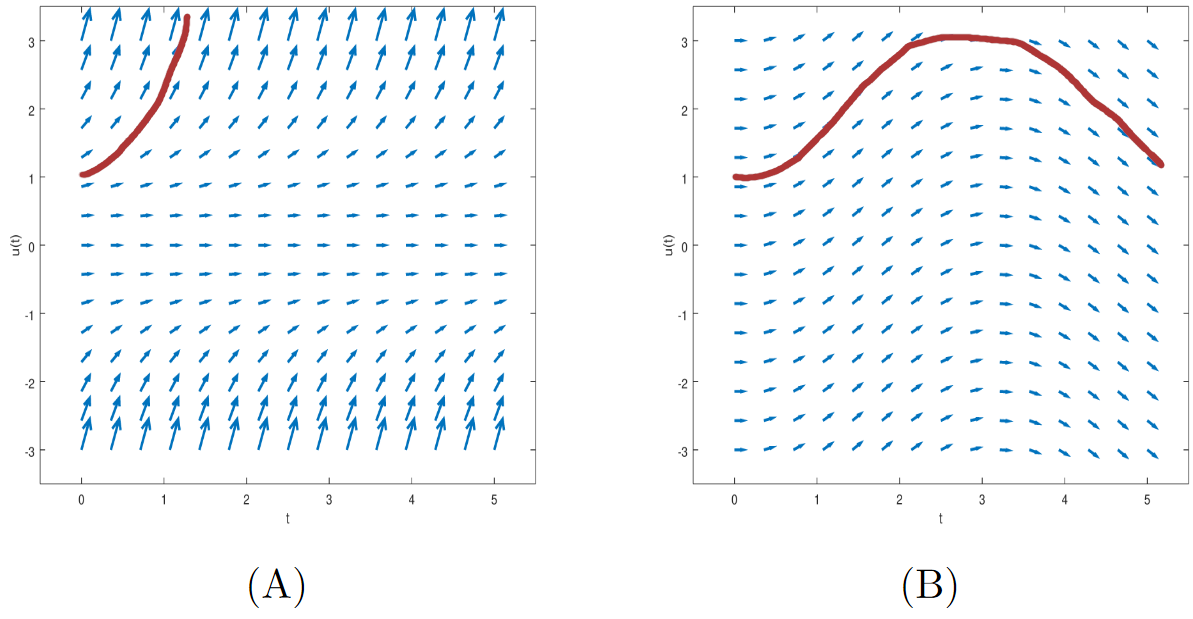
\includegraphics[width=0.9\linewidth]{Capture1x.png}
				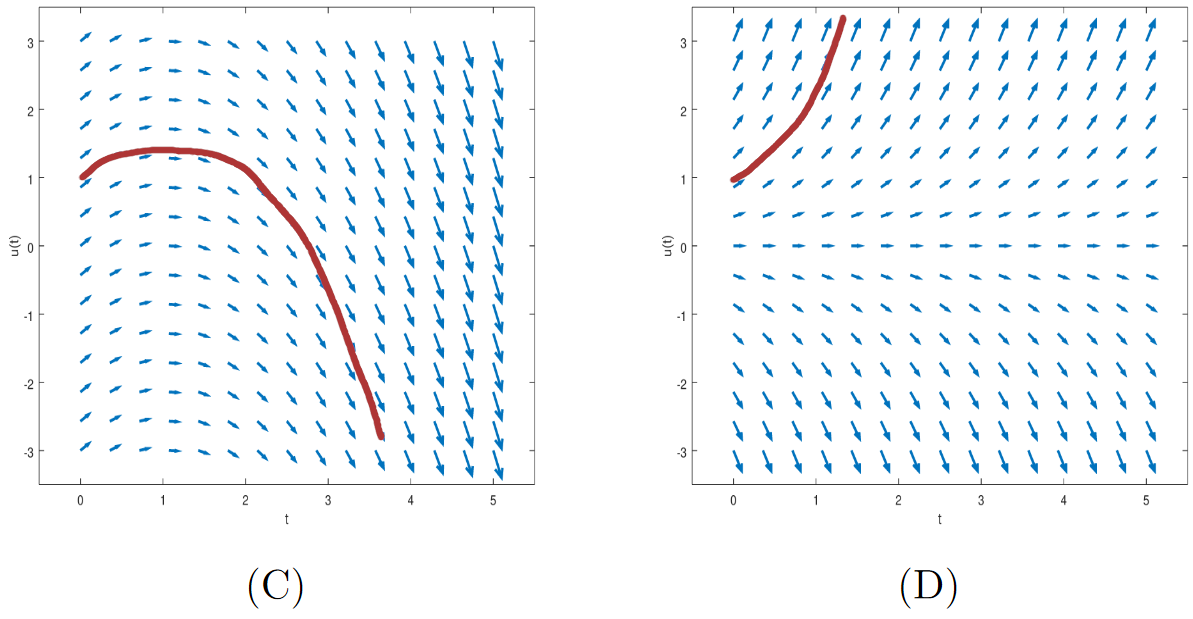
\includegraphics[width=0.9\linewidth]{Capture2x.png}
			\end{figure}
	\end{enumerate}
\end{exercise}

\end{document}
